\def\amadeusoverlay{%
  % highlighted components
  \foreach \n in {agent,req,state,router,rep,help} {\node[hl, fit=(\n)] {};}
  \node[hl, fit=(sensors)] {};
  % command: agent -> laptop -> relay -> DM -> camera
  \draw[flowreq] (agent.south) -- (agent |- mcp.north);
  \draw[flowreq] (req.east) -- (router.west);
  \draw[flowreq] (router.east) -- (rep.west);
  \draw[flowreq] (help.south) -- (help.south |- sensors.north);
  % reply: camera -> DM -> relay
  \draw[flowret] ([xshift=-5pt]help.south |- sensors.north) -- ([xshift=-5pt]help.south);
  \draw[flowret] ([yshift=-5pt]rep.west) -- ([yshift=-5pt]router.east);

  % reply: relay -> laptop -> state -> agent
  \draw[flowret] ([yshift=-5pt]router.west) -- ([yshift=-5pt]req.east);
  \draw[flowret] ([yshift=-5pt]req.west) .. controls +(-0.32,0) and +(-0.32,0) .. (state.west);
  \draw[flowret] ([xshift=-5pt]agent |- mcp.north) -- ([xshift=-5pt]agent.south);
  % numbered steps
  \node[badge] at (agent.north west) {1};
  \node[badge] at (state.east) {3};
  \node[badge] at ($(agent.south)!0.5!(agent |- mcp.north)+(0.4,0)$) {4};
  \node[badge] at (sensors.north west) {2};
  % labels
  \node[tag, anchor=south] at ([yshift=7pt]agent.north) {take\_camera\_image};
  \node[tag, anchor=north] at ([yshift=-3pt]mcp.south) {image saved};
  % step list
  \flowbadge{1}{Agent calls \code{take\_camera\_image}}
  \flowreqline{REQ\too ROUTER\too DM driver\too REP\too Helpers\too Sensors}
  \flowbadge{2}{Camera acquires}
  \flowretline{Sensors\too Helpers\too REP\too DM driver\too ROUTER\too REQ\too State}
  \flowbadge{3}{\code{image saved}}
  \flowbadge{4}{Result returns to the agent}
}
% Shared AMADEUS diagram. Compile one of the wrapper files:
%   amadeus_architecture.tex, amadeus_flow_microscope.tex, amadeus_flow_camera.tex
\providecommand{\amadeusoverlay}{}
\documentclass[tikz,border=6pt]{standalone}
\usepackage[T1]{fontenc}
\usepackage{lmodern}
\usepackage{enumitem}
\usetikzlibrary{positioning,fit,arrows.meta,calc}

\definecolor{laptop}{HTML}{2F6DB5}
\definecolor{pc}{HTML}{C0392B}
\definecolor{dm}{HTML}{7D3C98}
\definecolor{hw}{HTML}{4D4D4D}
\definecolor{net}{HTML}{1E8449}
\definecolor{flow}{HTML}{E67E22}

\pgfdeclarelayer{back}
\pgfdeclarelayer{midback}
\pgfdeclarelayer{mid}
\pgfsetlayers{back,midback,mid,main}

\newcounter{flowrow}
\newcommand{\flowrowpos}{%
  \stepcounter{flowrow}%
  \coordinate (fs) at ($(stepsorigin)+(0,-0.55*\value{flowrow})$);}
\newcommand{\flowbadge}[2]{\flowrowpos
  \node[badge] at (fs) {#1};
  \node[anchor=west, inner sep=0pt, font=\footnotesize] at ($(fs)+(0.45,0)$) {#2};}
\newcommand{\flowreqline}[1]{\flowrowpos
  \draw[flowreq] ($(fs)+(-0.25,0)$) -- ($(fs)+(0.25,0)$);
  \node[anchor=west, inner sep=0pt, font=\footnotesize] at ($(fs)+(0.45,0)$) {#1};}
\newcommand{\flowretline}[1]{\flowrowpos
  \draw[flowret] ($(fs)+(-0.25,0)$) -- ($(fs)+(0.25,0)$);
  \node[anchor=west, inner sep=0pt, font=\footnotesize] at ($(fs)+(0.45,0)$) {#1};}
\newcommand{\code}[1]{{\ttfamily #1}}
\newcommand{\too}{\,$\rightarrow$\,}
\newcommand{\note}[1]{\\[-1pt]{\scriptsize\color{black!55}#1}}

\begin{document}
\sffamily
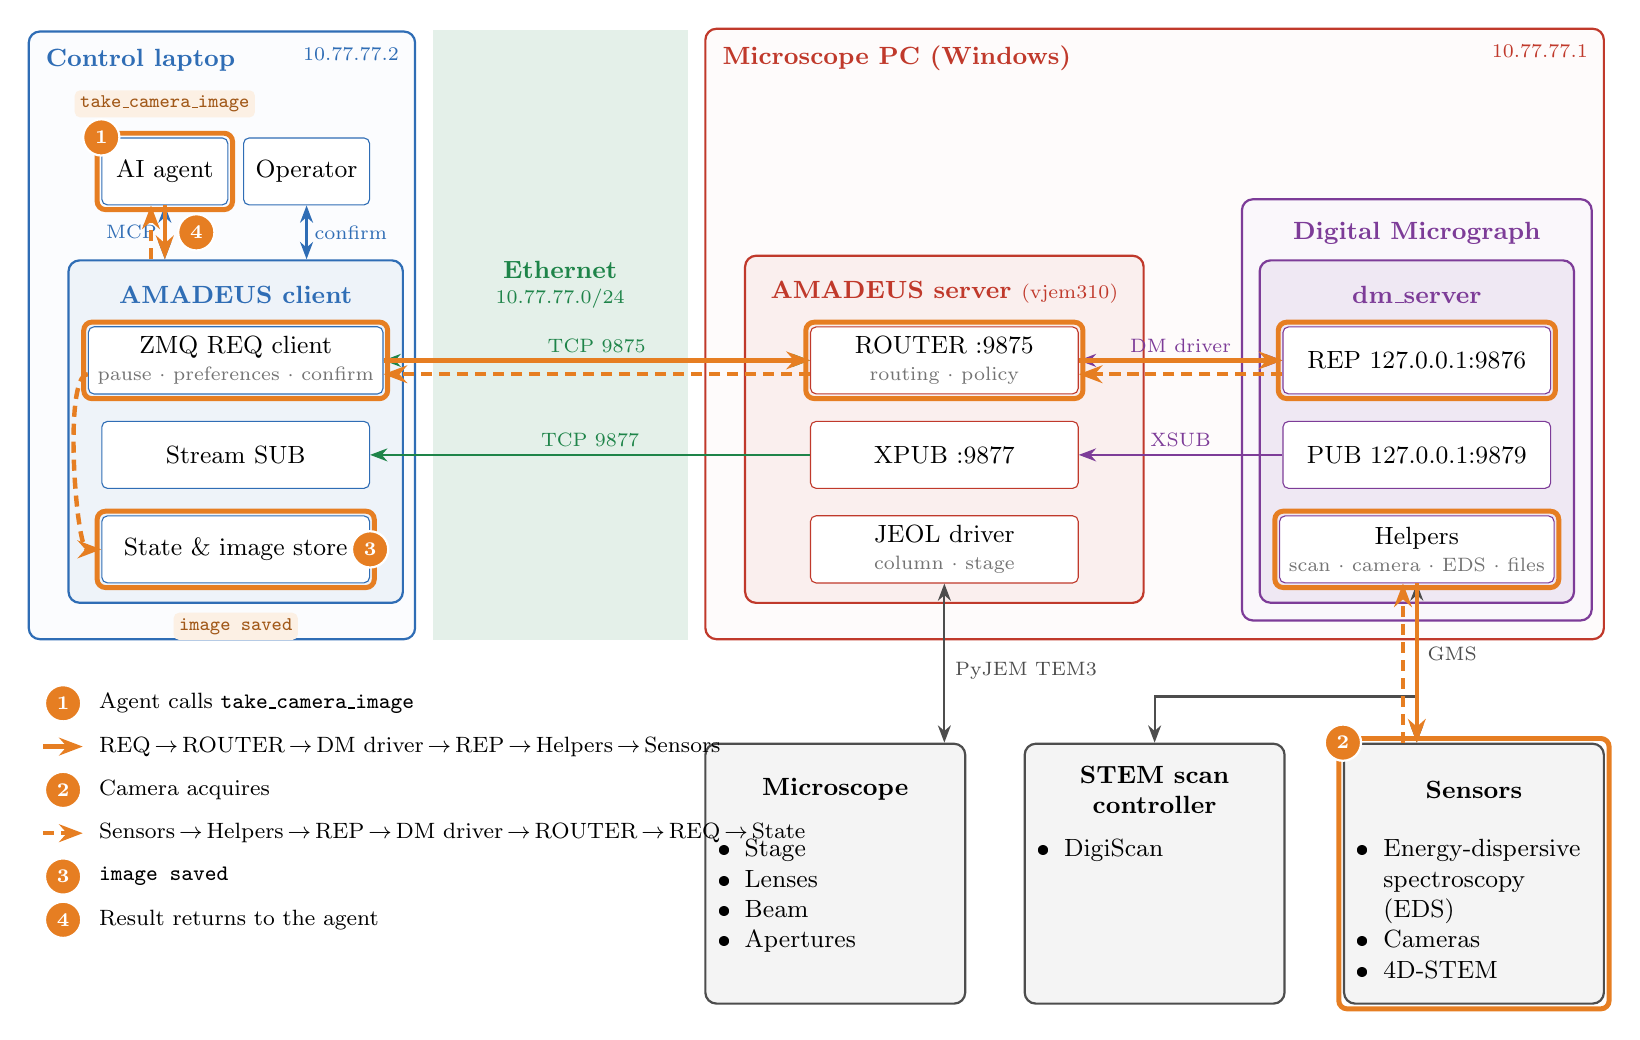
\begin{tikzpicture}[
  font=\small,
  >={Stealth[length=2.2mm]},
  comp/.style={draw, rounded corners=2pt, fill=white, minimum width=3.4cm,
               minimum height=0.85cm, align=center},
  user/.style={comp, minimum width=1.6cm},
  group/.style={draw, rounded corners=4pt, inner sep=8pt, thick},
  title/.style={font=\bfseries\small, anchor=south west, inner sep=2pt},
  sub/.style={font=\scriptsize, anchor=south east, inner sep=2pt},
  link/.style={->, thick},
  lbl/.style={font=\scriptsize, fill=white, inner sep=1.5pt},
  flowreq/.style={draw=flow, line width=1.6pt, ->, >={Stealth[length=3mm]}},
  flowret/.style={flowreq, dash pattern=on 4pt off 2.5pt},
  hl/.style={draw=flow, line width=1.8pt, rounded corners=3pt, inner sep=1.5pt},
  badge/.style={circle, fill=flow, draw=white, line width=0.8pt, text=white,
                font=\bfseries\scriptsize, inner sep=0pt, minimum size=4.6mm},
  tag/.style={font=\scriptsize\ttfamily, text=flow!70!black, fill=flow!12,
              rounded corners=2pt, inner sep=2pt},
]

% ---------------- Laptop ----------------
\node[user, draw=laptop] (agent) at (-0.9,7.0) {AI agent};
\node[user, draw=laptop] (operator) at (0.9,7.0) {Operator};
\node[title, text=laptop, anchor=south] (mcpt) at (0,5.25) {AMADEUS client};
\node[comp, draw=laptop] (req)   at (0,4.6) {ZMQ REQ client\note{pause $\cdot$ preferences $\cdot$ confirm}};
\node[comp, draw=laptop] (subc)  at (0,3.4) {Stream SUB};
\node[comp, draw=laptop] (state) at (0,2.2) {State \& image store};
\begin{pgfonlayer}{mid}
  \node[group, draw=laptop, fill=laptop!8, fit=(mcpt)(req)(subc)(state), inner sep=7pt] (mcp) {};
\end{pgfonlayer}
\draw[link, <->, laptop] (agent) -- node[lbl, left=1pt, fill=none] {MCP} (agent |- mcp.north);
\draw[link, <->, laptop] (operator) -- node[lbl, right=1pt, fill=none] {confirm} (operator |- mcp.north);

% ---------------- Microscope PC ----------------
\node[title, text=pc, anchor=south] (relayt) at (9,5.25) {AMADEUS server {\mdseries\scriptsize(vjem310)}};
\node[comp, draw=pc] (router) at (9,4.6) {ROUTER :9875\note{routing $\cdot$ policy}};
\node[comp, draw=pc] (xpub)   at (9,3.4) {XPUB :9877};
\node[comp, draw=pc] (hwb)    at (9,2.2) {JEOL driver\note{column $\cdot$ stage}};
\begin{pgfonlayer}{mid}
  \node[group, draw=pc, fill=pc!8, fit=(relayt)(router)(xpub)(hwb), inner sep=7pt] (relay) {};
\end{pgfonlayer}

\node[title, text=dm, anchor=south] (dmappt) at (15,6.0) {Digital Micrograph};
\node[title, text=dm, anchor=south] (dmst) at (15,5.25) {dm\_server};
\node[comp, draw=dm] (rep)  at (15,4.6) {REP 127.0.0.1:9876};
\node[comp, draw=dm] (pub)  at (15,3.4) {PUB 127.0.0.1:9879};
\node[comp, draw=dm] (help) at (15,2.2) {Helpers\note{scan $\cdot$ camera $\cdot$ EDS $\cdot$ files}};
\begin{pgfonlayer}{mid}
  \node[group, draw=dm, fill=dm!12, fit=(dmst)(rep)(pub)(help), inner sep=7pt] (dms) {};
\end{pgfonlayer}
\begin{pgfonlayer}{midback}
  \node[group, draw=dm, fill=dm!4, fit=(dmappt)(dms), inner sep=6pt] (dmapp) {};
\end{pgfonlayer}

\draw[link, <->, dm] (router) -- node[lbl, above=1pt, fill=none] {DM driver} (rep);
\draw[link, dm] (pub) -- node[lbl, above=1pt, fill=none] {XSUB} (xpub);

% ---------------- Machine frames (common height) ----------------
\coordinate (top) at (0,8.05);
\coordinate (bot) at (0,1.2);
\node[title, text=laptop, anchor=south west] (lapt) at ($(mcp.west |- top)+(-0.35,0.15)$) {Control laptop};
\node[title, text=pc, anchor=south west] (pct) at ($(relay.west |- top)+(-0.35,0.15)$) {Microscope PC (Windows)};
\begin{pgfonlayer}{back}
  \node[group, draw=laptop, fill=laptop!2, fit=(lapt)(mcp)(agent)(operator)(mcp.west |- bot), inner sep=4pt] (laptopbox) {};
  \node[group, draw=pc, fill=pc!2, fit=(pct)(relay)(dmapp)(relay.west |- bot)(dmapp.east |- top), inner sep=4pt] (pcbox) {};
\end{pgfonlayer}
\node[sub, text=laptop, anchor=north east] at ([shift={(-4pt,-4pt)}]laptopbox.north east) {10.77.77.2};
\node[sub, text=pc, anchor=north east] at ([shift={(-4pt,-4pt)}]pcbox.north east) {10.77.77.1};

% ---------------- Ethernet link ----------------
\begin{pgfonlayer}{back}
  \fill[net!12] ([xshift=6pt]laptopbox.north east) rectangle ([xshift=-6pt]pcbox.south west);
\end{pgfonlayer}
\coordinate (ethmid) at ($(laptopbox.east)!0.5!(pcbox.west)$);
\node[font=\bfseries\small, text=net] at ($(ethmid |- router)+(0,1.15)$) {Ethernet};
\node[font=\scriptsize, text=net] at ($(ethmid |- router)+(0,0.78)$) {10.77.77.0/24};

\draw[link, <->, net] (req) -- node[lbl, above=1pt, fill=none] {TCP 9875} (router);
\draw[link, net] (xpub) -- node[lbl, above=1pt, fill=none] {TCP 9877} (subc);

% ---------------- Instrument ----------------
\tikzset{
  devbox/.style={draw=hw, thick, rounded corners=4pt, fill=hw!6, inner sep=0pt},
  devtitle/.style={font=\bfseries\small, align=center, anchor=north, inner sep=0pt},
  devbody/.style={align=left, anchor=north, inner sep=0pt, text width=2.95cm},
}
\newcommand{\devlist}[1]{\begin{itemize}[leftmargin=1em, nosep, label=\textbullet]#1\end{itemize}}
\def\devw{3.3cm}\def\devh{3.3cm}\def\devgap{1.3cm}

% outer boxes (fixed size, aligned to the PC frame)
\path ($(pcbox.south west)+(0,-\devgap)$) coordinate (d1nw)
      ($(pcbox.south east)+(0,-\devgap)$) coordinate (d3ne);
\path ($(d1nw)!0.5!(d3ne)$) coordinate (d2n);
\begin{pgfonlayer}{mid}
  \node[devbox, minimum width=\devw, minimum height=\devh, anchor=north west] (scope) at (d1nw) {};
  \node[devbox, minimum width=\devw, minimum height=\devh, anchor=north] (scan) at (d2n) {};
  \node[devbox, minimum width=\devw, minimum height=\devh, anchor=north east] (sensors) at (d3ne) {};
\end{pgfonlayer}

% title band (two lines tall), then bodies at a common height
\node[devtitle, anchor=center] at ([yshift=-17pt]scope.north) {Microscope};
\node[devtitle, anchor=center] at ([yshift=-17pt]scan.north) {STEM scan\\controller};
\node[devtitle, anchor=center] at ([yshift=-17pt]sensors.north) {Sensors};
\node[devbody] at ([yshift=-30pt]scope.north) {\devlist{\item Stage \item Lenses \item Beam \item Apertures}};
\node[devbody] at ([yshift=-30pt]scan.north) {\devlist{\item DigiScan}};
\node[devbody] at ([yshift=-30pt]sensors.north) {\devlist{\item Energy-dispersive spectroscopy (EDS) \item Cameras \item 4D-STEM}};

\draw[link, <->, hw] (hwb.south) -- node[lbl, right=2pt, fill=none, pos=0.55] {PyJEM TEM3} (hwb.south |- scope.north);

\coordinate (split) at ($(help.south |- pcbox.south)!0.55!(help.south |- sensors.north)$);
\draw[link, <-, hw] (help.south) -- node[lbl, right=2pt, fill=none, pos=0.62] {GMS} (split);
\draw[link, hw] (split) -- (split |- sensors.north);
\draw[link, hw] (split) -| (scan.north);

% ---------------- Flow overlay (set by the variant file) ----------------
% Step list sits below the laptop; rows are added with \flowbadge / \flowreqline / \flowretline.
\coordinate (stepsorigin) at ($(laptopbox.south west)+(0.45,-0.25)$);
\setcounter{flowrow}{0}
\amadeusoverlay

\end{tikzpicture}
\end{document}

